\documentclass[a4paper, 12pt, french]{article}

\usepackage{babel}
\usepackage[T1]{fontenc}
\usepackage[utf8]{inputenc}
\usepackage{lmodern}

\usepackage{geometry}
\usepackage{graphicx}

% Define the margins
\geometry{top=2cm,left=2cm, right=2cm, bottom=2cm}

\title{Le jeu du taquin sous forme de système multi-agent}
\author{Guilhem \bsc{Marion} et Matthieu \bsc{Vieira}}
\date{juillet 2018}

\begin{document}

\maketitle

\section{Structure du programme}

Notre programme, écrit en Python 3, est composé de deux fichiers

Puzzle.py 

Agent.py, une classe pour chaque agent qui est créé, chaque agent est un thread

Dans la suite de ce rapport, nous prendrons pour chaque exemple une grille de taille $n \times n$ avec $n = 5$, mais ce paramètre est évidemment modifiable.

\section{Construction des cas}

\subsection{Le cas à un agent}

\begin{figure}[h]
	\centering
	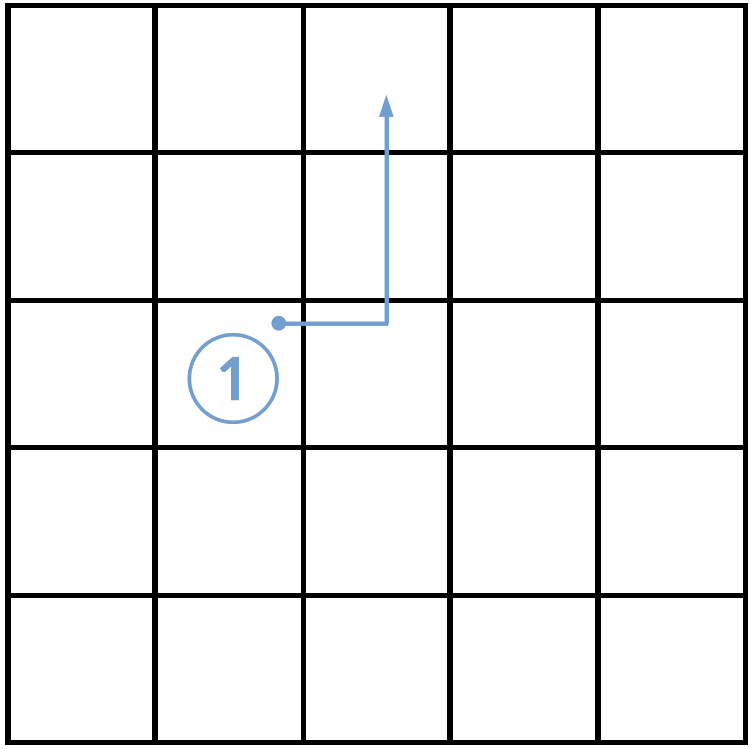
\includegraphics[width=200px]{images/base_case.png}
\end{figure}

C’est le cas le plus simple du programme. L'agent est seul sur la grille et a un objectif. Tant qu'il n'est pas sur sa case d'arrivée, l'agent calcule la distance par rapport à celle-ci pour chacune des cases sur laquelle il peut se déplacer. Dans le cas d'un quadrillage comme ici, la distance de Manhattan, donnée par la formule ci-dessous, est plus adaptée que la classique distance euclidienne.

\[
d(a, b) = |x_a - x_b| + |y_b - y_a|
\]

Dans le cas où deux directions sont possibles pour une distance de Manhattan, on choisit aléatoirement une des deux directions.



\begin{figure}[h]
	\centering
	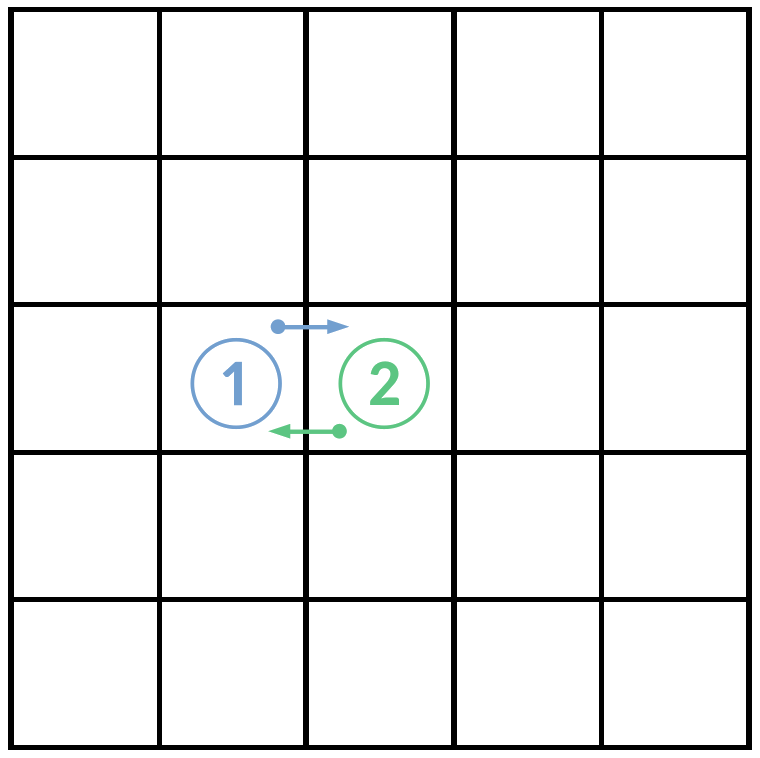
\includegraphics[width=200px]{images/switch.png}
\end{figure}

Contraites :

Chaque agent cognitif doit être doté de capacités de raisonnement et de réaction indépendantes, c'est le sens même de sa définition. Ici, chaque agent

\begin{figure}[h]
	\centering
	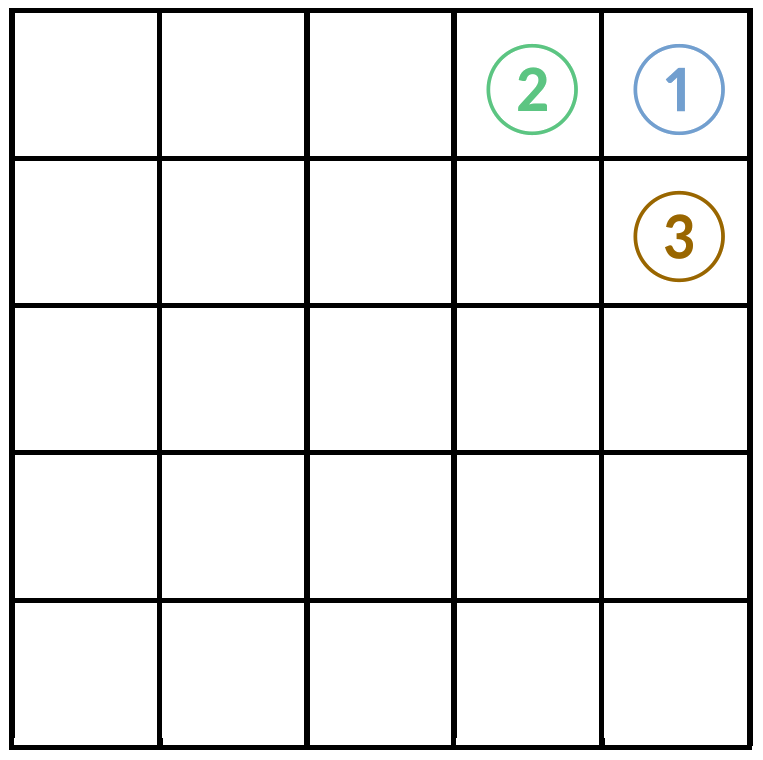
\includegraphics[width=200px]{images/3_agents.png}
\end{figure}

\begin{figure}[h]
	\centering
	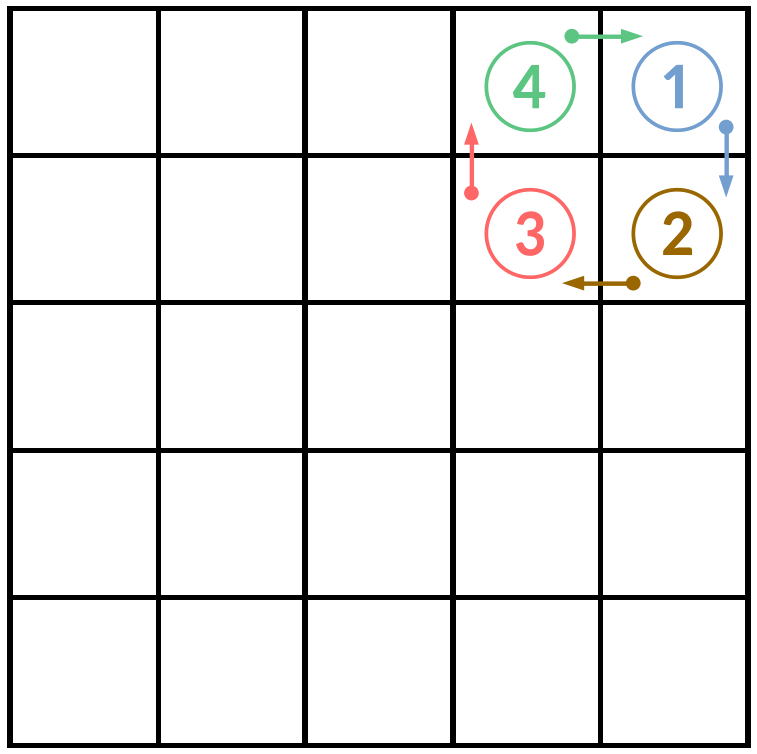
\includegraphics[width=200px]{images/4_agents.png}
\end{figure}

\begin{figure}[h]
	\centering
	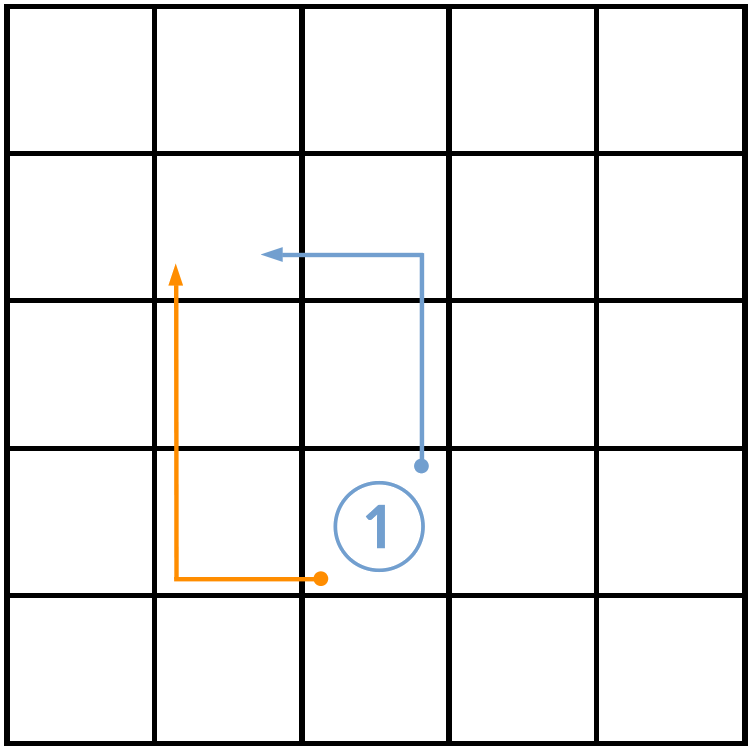
\includegraphics[width=200px]{images/manhattan_equal.png}
\end{figure}

\section{}

\end{document}
